\documentclass[conference]{IEEEtran}

\usepackage{amsmath,amssymb,amsfonts}
\usepackage{graphicx}
\usepackage{booktabs}
\usepackage{multirow}
\usepackage{array}
\usepackage{xcolor}
\usepackage{url}
\usepackage{cite}
\usepackage{balance}

\title{Focused Action Refinement for Frozen 1-bit Vision-Language-Action Models}

\author{
\IEEEauthorblockN{Miaomiao Dai, Yijie Liao, Weiyi Wang, Peilin Meng}
\IEEEauthorblockA{
Department of Electrical Engineering and Computer Science \\
University of Michigan \\
\texttt{\{dmmsjtu, lyjie, wweiyi, pailen\}@umich.edu}
}
}

\begin{document}

\maketitle


\begin{figure*}[t]
    \centering
    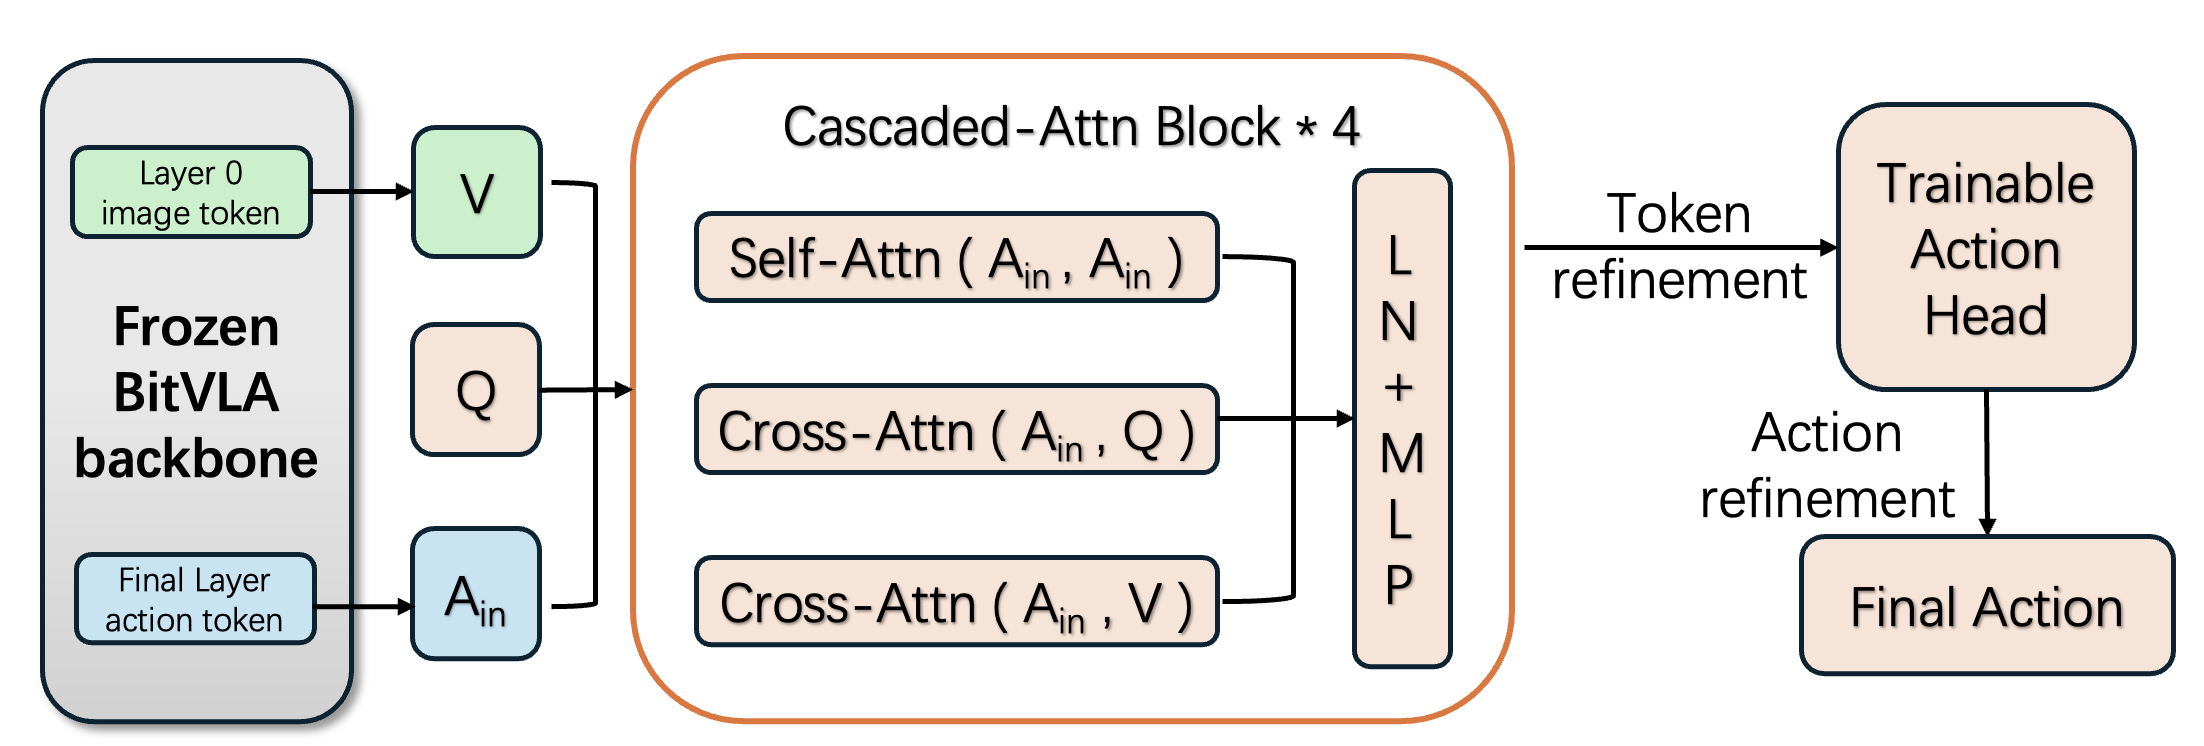
\includegraphics[width=\textwidth]{figures/architecture.png}
    \caption{Overview of the FAR framework. A frozen VLA backbone produces intermediate tokens and baseline actions. A lightweight refinement module processes these tokens through a cascaded attention encoder and produces a corrected action, which is bounded around the baseline via residual anchoring.}
    \label{fig:arch}
\end{figure*}

\begin{abstract}
Vision-Language-Action (VLA) models enable generalist robot control but remain costly to deploy. BitVLA reduces this cost via low-bit quantization, at the expense of action precision, especially in long-horizon manipulation tasks. We propose \textbf{Focused Action Refinement (FAR)}, a lightweight module that refines top-layer action features of a frozen 1-bit VLA backbone, improving action prediction without modifying backbone parameters. FAR combines (i) a triple-branch attention design that separates action self-attention, action--query cross-attention, and action--vision cross-attention into independent softmax branches, (ii) a patch-level top-$k$ visual selection paired with channel gating, and (iii) a dual-level residual anchoring strategy that bounds refinement for stable execution. On LIBERO-Long, FAR improves success rate from 85.8\% to 88.6\%, with larger gains on multi-object tasks. The module adds only 120M parameters on top of a 3.5B frozen backbone (3.4\%), offering an efficient way to recover precision loss from extreme quantization.
\end{abstract}

\section{Introduction}
Vision-Language-Action (VLA) models unify visual perception, language conditioning, and robot control into a single policy, enabling a wide range of manipulation tasks under natural language instructions. Recent systems such as OpenVLA and $\pi_0$ demonstrate that a single model can generalize across diverse manipulation tasks. However, their practical deployment remains constrained by model scale, as high-capacity VLAs require substantial memory and computational resources \cite{black2024pi0, kim2024openvla, zitkovich2023rt}.

BitVLA addresses this challenge through aggressive quantization, reducing the backbone to 1-bit weights with 8-bit activations while maintaining competitive performance. Despite this efficiency gain, quantization introduces systematic degradation in action precision, particularly in long-horizon manipulation tasks involving multiple objects and spatial reasoning \cite{wang2025bitvla}. 

This raises a key question: \emph{can we recover the lost precision of a quantized VLA without retraining or modifying the backbone?}

In this work, we propose \textbf{Focused Action Refinement (FAR)}, a lightweight sidecar module that improves action prediction of a frozen 1-bit VLA policy. Instead of relearning the full control policy, FAR operates on top-layer action representations and selectively refines them using multimodal interactions with visual features. The refinement is explicitly constrained to a bounded residual around the baseline action, so the closed-loop behavior cannot drift far from the frozen policy even when the refinement output is noisy.

The central idea is to make refinement structured and selective. Drawing on FocusVLA's modality-cascaded design \cite{zhang2026focusvla}, FAR disentangles action self-attention, action--query cross-attention, and action--vision cross-attention into three independent softmax branches, preventing the query-side shortcut that can arise when modalities share a single attention. In addition, it employs patch-level top-$k$ selection and channel gating to attend to task-relevant visual evidence, and a dual-level residual anchoring mechanism to bound refinement at both the feature and action levels.

This work has two parts, aligned with the course's \emph{reproduction + extension} deliverable structure:
\begin{itemize}
    \item \textbf{Reproduction.} We first reproduce the LIBERO-Long rollout result of the base paper (BitVLA \cite{wang2025bitvla}) under the authors' official evaluation protocol, verifying the published baseline and establishing a trustworthy reference point for our extension.
    \item \textbf{Algorithmic extension.} We then propose Focused Action Refinement (FAR) as a new component on top of the reproduced baseline, and evaluate it under the same protocol to quantify its improvement.
\end{itemize}

Our contributions are summarized as follows:
\begin{itemize}
    \item We propose a frozen-backbone action refinement module for quantized VLA policies, improving action precision without modifying backbone parameters.
    \item We introduce a triple-branch attention mechanism that enforces structured interactions between action, query, and visual tokens, mitigating shortcut learning.
    \item We design a visual refinement strategy combining patch-level top-$k$ selection with channel gating, together with dual-level residual anchoring to ensure stable closed-loop execution.
    \item We demonstrate improvements on LIBERO-Long, increasing success rate from 85.8\% to 88.6\%, with the largest gains on multi-object manipulation tasks \cite{liu2023libero}.
\end{itemize}

\section{Related Work}

\subsection{Vision-Language-Action Models}
Vision-Language-Action (VLA) models connect language-conditioned perception with continuous robot control, enabling generalist manipulation policies under natural language instructions. OpenVLA demonstrates that large pretrained multimodal architectures can be adapted into unified robot policies, achieving strong generalization across tasks \cite{kim2024openvla}. BitVLA extends this line of work toward efficient deployment by applying aggressive low-bit quantization, significantly reducing memory and computation while maintaining competitive performance on LIBERO benchmarks \cite{wang2025bitvla}. In parallel, models such as $\pi_0$ explore alternative policy representations, including flow-matching-based generation for manipulation tasks \cite{black2024pi0}. 
Despite these advances, a key challenge remains: how to preserve action accuracy under strict efficiency constraints, especially in long-horizon and multi-object manipulation settings.

\subsection{Efficient Adaptation of Large Models}
Parameter-efficient adaptation methods, such as LoRA, reduce the number of trainable parameters during fine-tuning by introducing low-rank updates into pretrained models \cite{hu2022lora}. Similar approaches have been widely applied in vision-language and robotics models to enable efficient adaptation without full retraining. However, these methods still modify the backbone representations, which may alter the deployment characteristics of highly optimized models such as quantized VLAs.
In contrast, our approach preserves a strictly frozen backbone and shifts all adaptation into a separate refinement module. This design is particularly relevant for quantized policies, where maintaining the original inference cost and numerical behavior is critical.

\subsection{Structured Attention for Multimodal Policies}
Structured attention mechanisms in multimodal models have been shown to mitigate shortcut learning and improve cross-modal grounding. The Multimodal Transformer introduced cross-modal attention for unaligned multimodal sequences \cite{tsai2019multimodal}, and subsequent work has studied how to control information flow between modalities in VLA policies. Most directly related to our work, FocusVLA \cite{zhang2026focusvla} proposed a modality-cascaded attention with patch-level focus and channel gating for end-to-end VLA training, showing that explicit modality separation and selective visual utilization substantially improve action prediction.

Our method adapts FocusVLA's attention design to a frozen-backbone inference setting. Rather than retraining a full VLA policy, we introduce a lightweight refinement module on top of a quantized BitVLA backbone. The module inherits the cascaded attention and top-$k$ plus channel-gate visual selection from FocusVLA, but operates purely as a post-hoc corrector that never modifies the backbone's 1-bit weights. In this sense FAR sits closer to a bounded residual corrector than to a standalone policy.

\section{Algorithmic Extension: FAR}
\subsection{Problem Setup}
We consider a frozen quantized Vision-Language-Action (VLA) policy
\begin{equation}
f_{\text{base}} : (I, w, p, l) \mapsto a_{\text{base}},
\end{equation}
where $I$ denotes RGB observations, $w$ wrist-view images, $p$ proprioception, and $l$ the language instruction. The model predicts chunked actions $a_{\text{base}} \in \mathbb{R}^{K \times A}$ with horizon $K=8$ and action dimension $A=7$.
In addition to the final action, the frozen backbone exposes intermediate representations:
\begin{itemize}
    \item early visual tokens $H_0 \in \mathbb{R}^{B \times N_v \times D}$,
    \item top-layer action tokens $H_{\text{top}} \in \mathbb{R}^{B \times K \times A \times D}$,
\end{itemize}
where $D$ is the hidden dimension and $N_v$ is the number of visual tokens.
Our goal is to learn a refinement function
\begin{equation}
a_{\text{final}} = g(H_0, H_{\text{top}}, a_{\text{base}})
\end{equation}
that improves action accuracy while keeping the backbone fully frozen.

\subsection{FAR Framework}
The proposed Focused Action Refinement (FAR) module operates as a lightweight sidecar on top of the frozen backbone (Fig.~\ref{fig:arch}). It consists of three stages: (1) feature extraction, (2) token refinement via cascaded attention, and (3) bounded action correction.
We first project the extracted features into a refinement space of dimension $R$:
\begin{align}
A &= W_A H_{\text{top}} + E_{\text{chunk}} + E_{\text{dim}}, \\
Q &= Q_{\text{emb}} + E_{\text{chunk}}, \\
V &= W_V H_0,
\end{align}
where $A \in \mathbb{R}^{B \times 56 \times R}$ are flattened action tokens, $Q \in \mathbb{R}^{B \times K \times R}$ are learned chunk query tokens, and $V \in \mathbb{R}^{B \times N_v \times R}$ are visual tokens.

\subsection{Cascaded Attention Refinement}
A key design in FAR is to decouple multimodal interactions into separate attention branches. Instead of mixing all tokens in a single attention, we explicitly model:
\begin{align}
H_A &= \text{SelfAttn}(A_{\text{in}}, A_{\text{in}}), \\
H_Q &= \text{CrossAttn}(A_{\text{in}}, Q), \\
H_V &= \text{CrossAttn}(A_{\text{in}}, V).
\end{align}
Each branch uses an independent softmax, preventing competition between modalities and ensuring that visual information is explicitly incorporated.
The outputs are fused as:
\begin{align}
H_{\text{fuse}} &= \text{MLP}([\text{LN}(H_A), \text{LN}(H_Q), \text{LN}(H_V)]), \\
A_{\text{out}} &= A_{\text{in}} + H_{\text{fuse}} + \text{FFN}(A_{\text{in}} + H_{\text{fuse}}).
\end{align}
To improve spatial selectivity, we restrict attention to the top-$k$ visual tokens:
\begin{equation}
\tilde{S}_{ij} =
\begin{cases}
S_{ij}, & j \in \text{TopK}(S_i), \\
-\infty, & \text{otherwise},
\end{cases}
\end{equation}
followed by
\begin{equation}
H_V^{\text{raw}} = \text{softmax}(\tilde{S}) V.
\end{equation}
We further apply channel-wise gating:
\begin{equation}
H_V = H_V^{\text{raw}} \odot \sigma(\text{MLP}(A_{\text{in}})),
\end{equation}
which enables fine-grained filtering of visual features.

\subsection{Action Decoding and Anchoring}
The refined latent is reshaped as
\begin{equation}
z_{\text{action}} \in \mathbb{R}^{B \times K \times A \times R}.
\end{equation}
We apply token-level refinement:
\begin{equation}
\Delta h = \delta \cdot \tanh(\text{MLP}([z_{\text{action}}, H_{\text{top}}])),
\end{equation}
and obtain
\begin{equation}
H_{\text{refined}} = H_{\text{top}} + \Delta h.
\end{equation}
The final action is predicted as
\begin{equation}
a_{\text{refine}} = \text{Head}(H_{\text{refined}}),
\end{equation}
and anchored to the baseline:
\begin{equation}
a_{\text{final}} = a_{\text{base}} + \rho \cdot \tanh(a_{\text{refine}} - a_{\text{base}}).
\end{equation}
This dual-level residual design ensures that refinement remains stable and bounded.


\section{Experimental Setup}
\subsection{Dataset and Benchmark}
We evaluate our method on the LIBERO-Long benchmark, using the \texttt{libero\_10\_no\_noops} dataset for training and the \texttt{libero\_10} suite for rollout evaluation. The benchmark consists of 10 long-horizon manipulation tasks, each evaluated with 50 trials, resulting in 500 episodes in total.

The policy takes as input $224 \times 224$ RGB observations from both agent-view and wrist-view cameras, along with proprioceptive state and a language instruction. It predicts an 8-step chunked action sequence with 7 DoF, executed in an open-loop manner.

\subsection{Model Configuration}
We use a frozen BitVLA backbone pretrained on LIBERO-Long. The backbone is a 30-layer model with approximately 3.5B parameters under low-bit quantization.

The FAR module introduces approximately 120M trainable parameters (3.4\% of the backbone size). Key hyperparameters are summarized in Table~\ref{tab:hyper}.

\begin{table}[t]
\centering
\caption{Main FAR hyperparameters.}
\label{tab:hyper}
\begin{tabular}{lc}
\toprule
Parameter & Value \\
\midrule
Backbone hidden dim $D$ & 2560 \\
Refinement dim $R$ & 640 \\
Heads & 8 \\
Layers & 4 \\
Chunk size & 8 \\
Action dimension & 7 \\
Top-$k$ patches & 256 \\
Token scale $\delta$ & 0.30 \\
Pose scale $\rho$ & 0.10 \\
\bottomrule
\end{tabular}
\end{table}

\subsection{Training Details}
We adopt a strict frozen-backbone setting:
\begin{equation}
(H_0, H_{\text{top}}, a_{\text{base}}) = f_{\text{base}}(x),
\end{equation}
where extracted features are detached from gradient flow.

The final action is modeled as a bounded residual:
\begin{equation}
a_{\text{final}} = a_{\text{base}} + \rho \cdot \tanh(a_{\text{refine}} - a_{\text{base}}).
\end{equation}

The training objective combines pose regression and gripper classification:
\begin{align}
\mathcal{L}_{\text{pose}} &= \text{SmoothL1}(a_{\text{pose}}, a_{\text{gt}}), \\
\mathcal{L}_{\text{grip}} &= \text{BCE}(a_{\text{grip}}, a_{\text{gt}}), \\
\mathcal{L} &= \mathcal{L}_{\text{pose}} + \lambda \mathcal{L}_{\text{grip}},
\end{align}
with $\lambda = 1.0$.

We optimize the model using AdamW with separate learning rates for the encoder ($2\times10^{-4}$) and action head ($5\times10^{-5}$), and apply cosine decay with linear warmup (500 steps over 10k total steps).

Training uses batch size 8 with gradient accumulation (effective batch size 16). Gradient clipping ($\tau=1.0$) and residual anchoring are applied to ensure stability. The full 10,000-step training completes in approximately 3 hours on a single NVIDIA RTX 5090 (32\,GB). Closed-loop rollout evaluation on all 500 LIBERO-Long episodes takes approximately 2.7 hours on the same hardware.

\section{Results}

\subsection{Paper Reproduction}

As the first deliverable, we reproduce the LIBERO-Long rollout result of the base paper (BitVLA \cite{wang2025bitvla}) using the authors' official evaluation script at \texttt{repos/BitVLA/.../run\_libero\_eval\_bitnet.py}. We run 500 rollout episodes (10 tasks $\times$ 50 trials, \texttt{seed=7}) on the official \texttt{ft-libero-long-bf16} checkpoint with \texttt{center\_crop=True}, \texttt{num\_open\_loop\_steps=8}, and \texttt{num\_steps\_wait=10} --- matching the BitVLA paper's evaluation protocol exactly. Our reproduction obtains $\mathbf{85.8\%}$ (429/500) success, closely matching the BitVLA paper's reported ``without robotics pretraining'' result of 87.6\% on the same suite. The small gap is consistent with simulator non-determinism (MuJoCo / driver version) across independent runs. This reproduced baseline serves as the reference point against which our extension is measured.

\subsection{Extension Results}

Table~\ref{tab:overall} compares the reproduced baseline against our proposed extension, FAR, under the same 500-episode protocol.

\begin{table}[t]
\centering
\caption{Overall success rate: reproduced baseline vs. our extension.}
\label{tab:overall}
\begin{tabular}{lccc}
\toprule
Method & Success & Total & Success Rate \\
\midrule
BitVLA baseline (reproduced) & 429 & 500 & 85.8\% \\
FAR (our extension)          & 443 & 500 & \textbf{88.6\%} \\
\bottomrule
\end{tabular}
\end{table}

FAR improves the overall success rate by $\mathbf{+2.8}$ percentage points (14 additional successful episodes) on top of the reproduced baseline. This demonstrates that a lightweight refinement module can recover part of the precision loss introduced by aggressive quantization without modifying the frozen backbone.

\subsection{Per-Task Analysis}
Table~\ref{tab:per_task} reports per-task performance across all tasks.
\begin{table}[t]
\centering
\caption{Per-task performance on LIBERO-Long.}
\label{tab:per_task}
\small
\setlength{\tabcolsep}{4pt}
\begin{tabular}{lccc}
\toprule
Task & Baseline & FAR & $\Delta$ \\
\midrule
Task 0 & 84\% & 92\% & +8 \\
Task 1 & 96\% & 100\% & +4 \\
Task 2 & 96\% & 92\% & -4 \\
Task 3 & 94\% & 86\% & -8 \\
Task 4 & 76\% & 92\% & +16 \\
Task 5 & 100\% & 98\% & -2 \\
Task 6 & 68\% & 80\% & +12 \\
Task 7 & 82\% & 88\% & +6 \\
Task 8 & 72\% & 74\% & +2 \\
Task 9 & 90\% & 84\% & -6 \\
\bottomrule
\end{tabular}
\end{table}

FAR improves performance on the majority of tasks, with the largest gains on Task 4 (+16) and Task 6 (+12), which correspond to more challenging scenarios involving multi-object interactions and spatial reasoning. This suggests that the refinement module is particularly effective when precise visual grounding is required.

Performance decreases are observed on a few tasks (e.g., Task 3 and Task 9), indicating that refinement is not uniformly beneficial and may occasionally introduce over-correction when the baseline policy is already near-optimal.

Overall, FAR improves performance primarily on harder tasks while maintaining competitive performance on easier ones, supporting the hypothesis that refinement is most effective when quantization errors accumulate in long-horizon or spatially complex scenarios.

\section{Discussion}

FAR improves performance primarily on tasks involving multi-object interactions and spatial reasoning. In particular, Tasks 4 and 6 show the largest gains (+16 and +12), suggesting that the proposed visual focus mechanism effectively recovers spatial precision lost due to quantization. By selectively attending to relevant regions, the model is better able to ground actions in complex scenes.

At the same time, performance degrades on a few tasks (e.g., Task 3 and Task 9), which involve tighter temporal dependencies. In these cases, refinement may introduce slight over-correction, interfering with stable execution when the baseline policy is already well-optimized.

The patch-level top-$k$ selection plays a key role in reducing noise from irrelevant regions, improving robustness in cluttered environments. However, aggressive filtering may also remove useful contextual information, which can contribute to performance drops in certain scenarios.

Residual anchoring ensures that the refined action remains close to the baseline:
\begin{equation}
|a_{\text{final}} - a_{\text{base}}| \le \rho
\end{equation}
This constraint prevents large deviations and maintains rollout stability. Empirically, FAR improves performance without introducing catastrophic failures.

Finally, FAR remains computationally efficient, introducing only 120M trainable parameters (3.4\% of the backbone) and requiring approximately 3 hours of training on a single RTX 5090. This highlights that meaningful performance gains can be achieved through lightweight refinement rather than full-model retraining.

\subsection{Limitations and Future Directions}
FAR operates under a strictly frozen backbone, which fundamentally bounds its achievable performance by the information already encoded in $H_0$ and $H_{\text{top}}$. If aggressive 1-bit quantization has destroyed information that is simply not present in these features, no post-hoc refinement can recover it. A complementary direction is end-to-end joint training of the backbone and refinement module with action supervision, which could in principle recover more of the performance gap to full-precision VLAs, at the cost of losing the drop-in deployability and 1-bit memory footprint that motivated this work.

Our evaluation uses a single random seed (\texttt{seed=7}) and a single LIBERO suite (LIBERO-Long). Multi-seed variance is not measured, and generalization to LIBERO-Spatial, LIBERO-Object, LIBERO-Goal, and real-robot execution remains untested. We also observe a persistent offline--online gap: pose MAE on held-out demonstrations does not reliably predict closed-loop rollout success, so checkpoint selection must be done via costly rollout evaluation rather than cheap offline metrics. Finally, FAR assumes access to the backbone's intermediate activations $H_0$ and $H_{\text{top}}$; closed-source or API-only VLAs that expose only the final action would require additional feature-probing effort before FAR can be applied.

\section{Conclusion}

We present Focused Action Refinement (FAR), a lightweight module for improving frozen 1-bit Vision-Language-Action models. By combining structured attention, visual focus, and bounded residual refinement, FAR recovers part of the precision loss introduced by aggressive quantization.

Experiments on LIBERO-Long demonstrate consistent improvements, particularly on tasks requiring spatial reasoning and multi-object interaction, while maintaining low computational overhead.

Future work includes (i) extending FAR to other frozen VLA backbones such as OpenVLA and $\pi_0$ under various quantization schemes, (ii) exploring joint backbone--refinement training to push absolute performance further while preserving deployment efficiency, and (iii) developing time-adaptive refinement schedules (e.g., a chunk-step-dependent $\rho$) to reduce over-correction on pose-sensitive closure tasks.


\bibliographystyle{IEEEtran}
\bibliography{references}

\end{document}
